\subsection{Types of Flow Conditions}

\begin{frame}[fragile,containsverbatim]\frametitle{Types of Flow Conditions}

\vspace{0.1in}
\centering
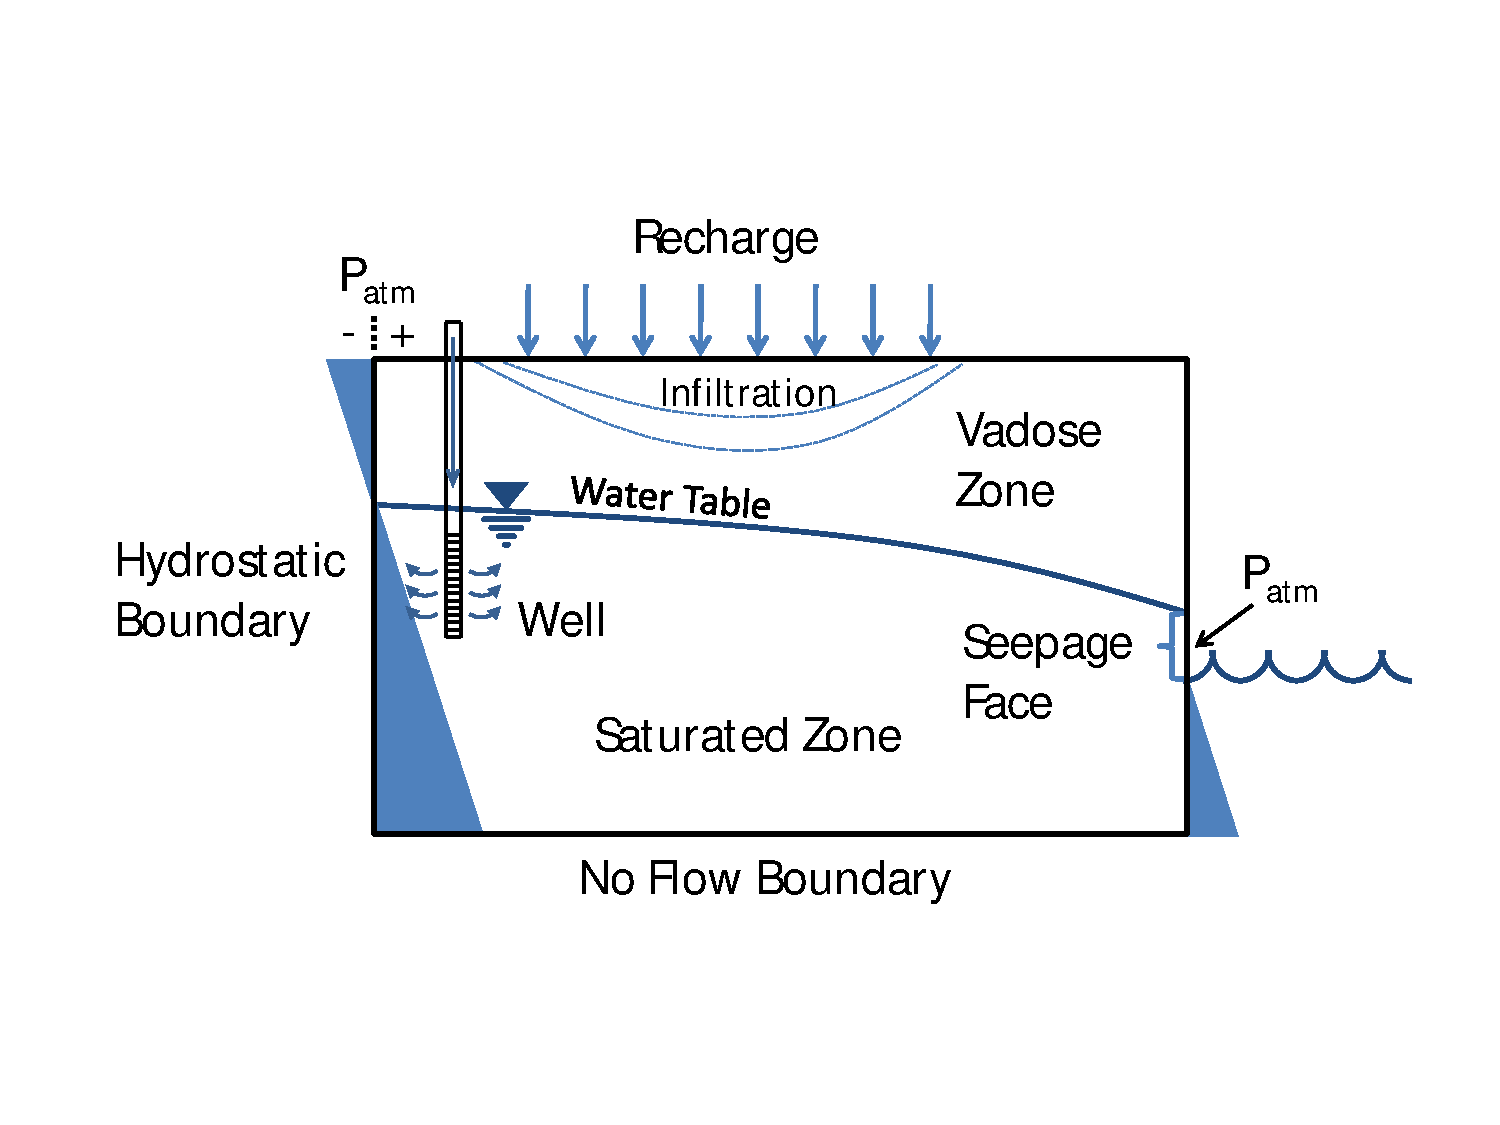
\includegraphics[width=0.9\linewidth]{./flow_bcs_with_well}
%\vspace{-0.5in}
\small 
\begin{tabbing}
\verb|DIRICHLET        |	\= Specified pressure across region\\
\verb|HYDROSTATIC|	      \> Hydrostatic pressure profile across region\\
\verb|SEEPAGE|	         	\> Hydrostatic with outflow only above water table\\
\verb|NEUMANN|			      \> Darcy flux across boundary [L/T]\\
\verb|MASS_RATE|	      	\> Mass injection/extraction rate [M/T]\\
\verb|VOLUMETRIC_RATE|	  \> Volumetric injection/extraction rate [L$^3$/T]\\
\end{tabbing}

\end{frame}

